This section describes the integration of the IMP solution presented in section 5.1 using the same messaging system as described in section 4.2.

\subsection{Integration Overview}

\begin{center}
    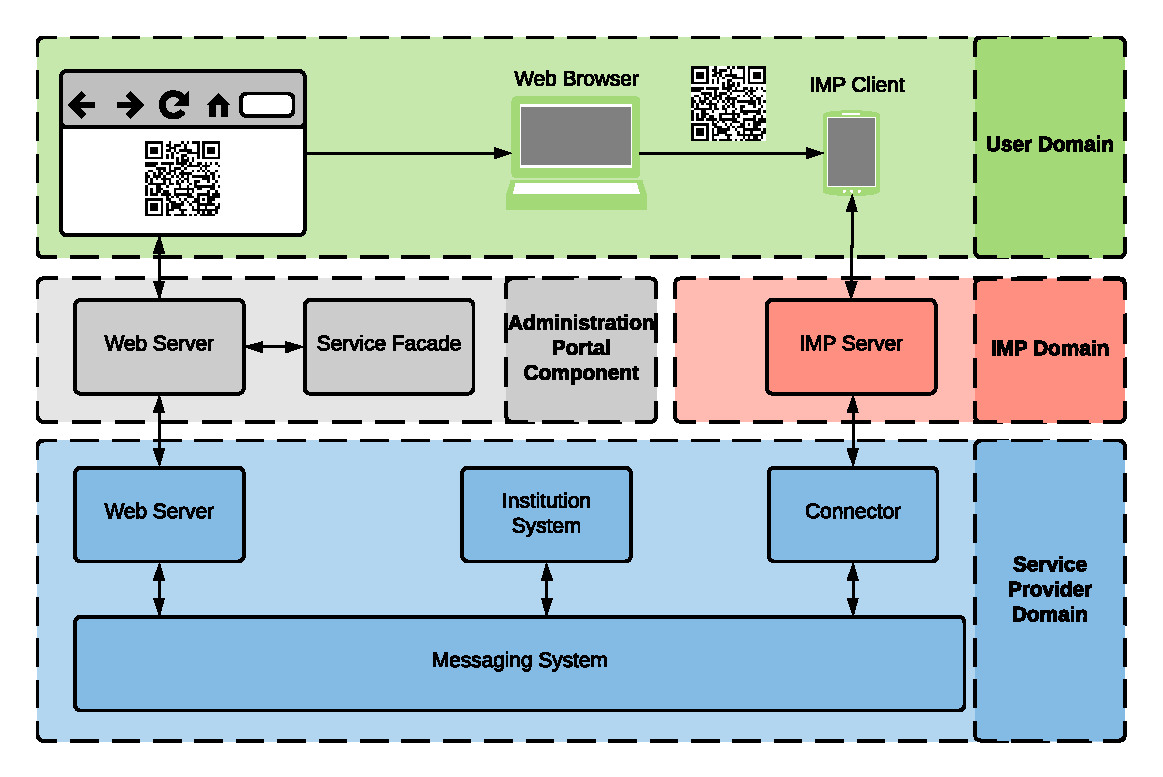
\includegraphics[scale=0.6]{Diagrams/Integration Architecture 2/Technological Integration/1. Integration Overview.pdf}
\end{center}

To implement the IMP solution, a connector is included in the existing system architecture of each institution as well as the messaging system described in section 4.2. Instead of the web server and service facade in the portal domain, the messaging system is connected to the web server and institution system of the institution domain.

\begin{center}
    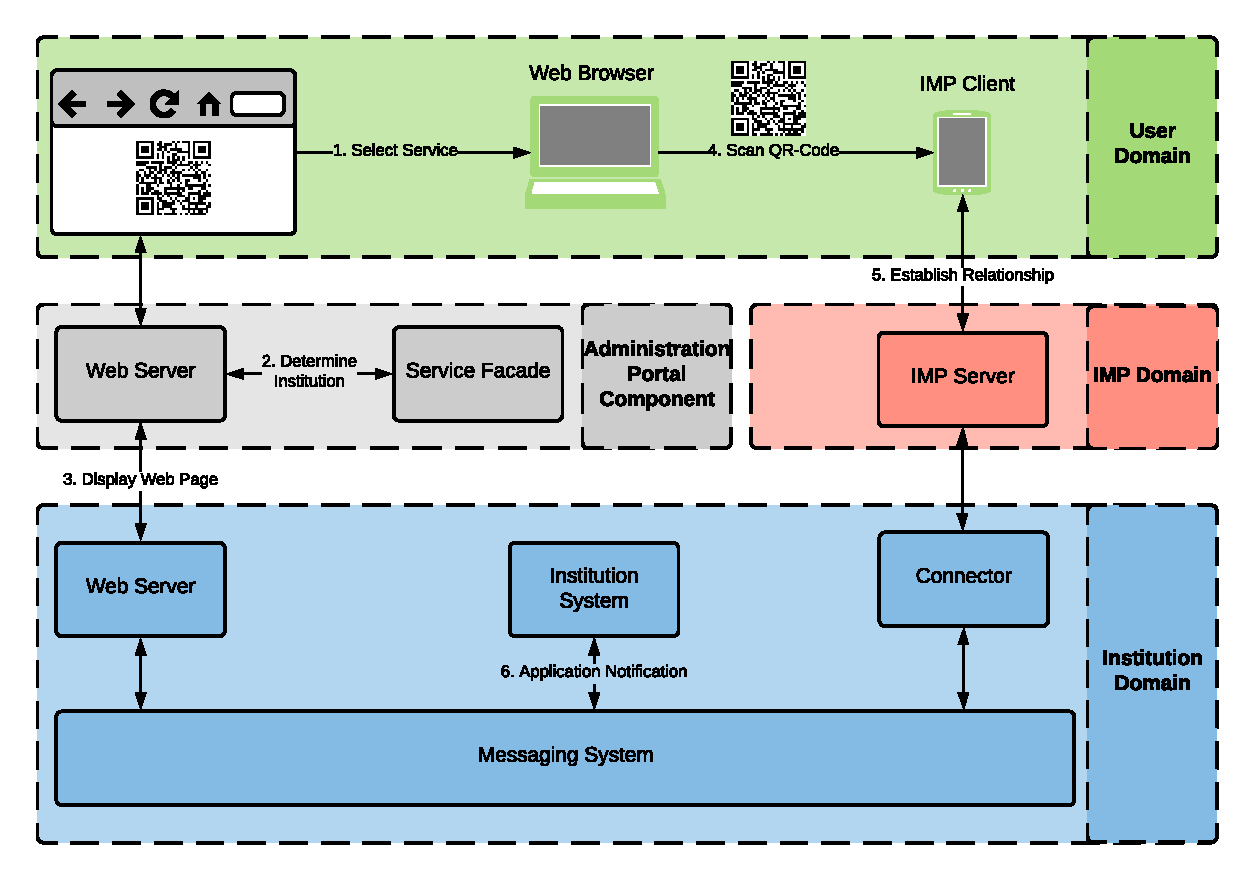
\includegraphics[scale=0.6]{Diagrams/Integration Architecture 2/Technological Integration/3. Application Overview.pdf}
\end{center}

Institutions are able to process a predetermined set of administrative services. For each service, the institution can once create a relationship template and store them as QR code on their web page. 

Users visiting an administration portal can select an administrative service, specify their home address and be forwarded to the web page of the respective institution. After scanning the appropriate QR code with the IMP client, the user can fill in the requested attributes and send the relationship request. After the relationship is established, the institution is notified and starts processing the application utilizing the shared attributes.

\begin{center}
    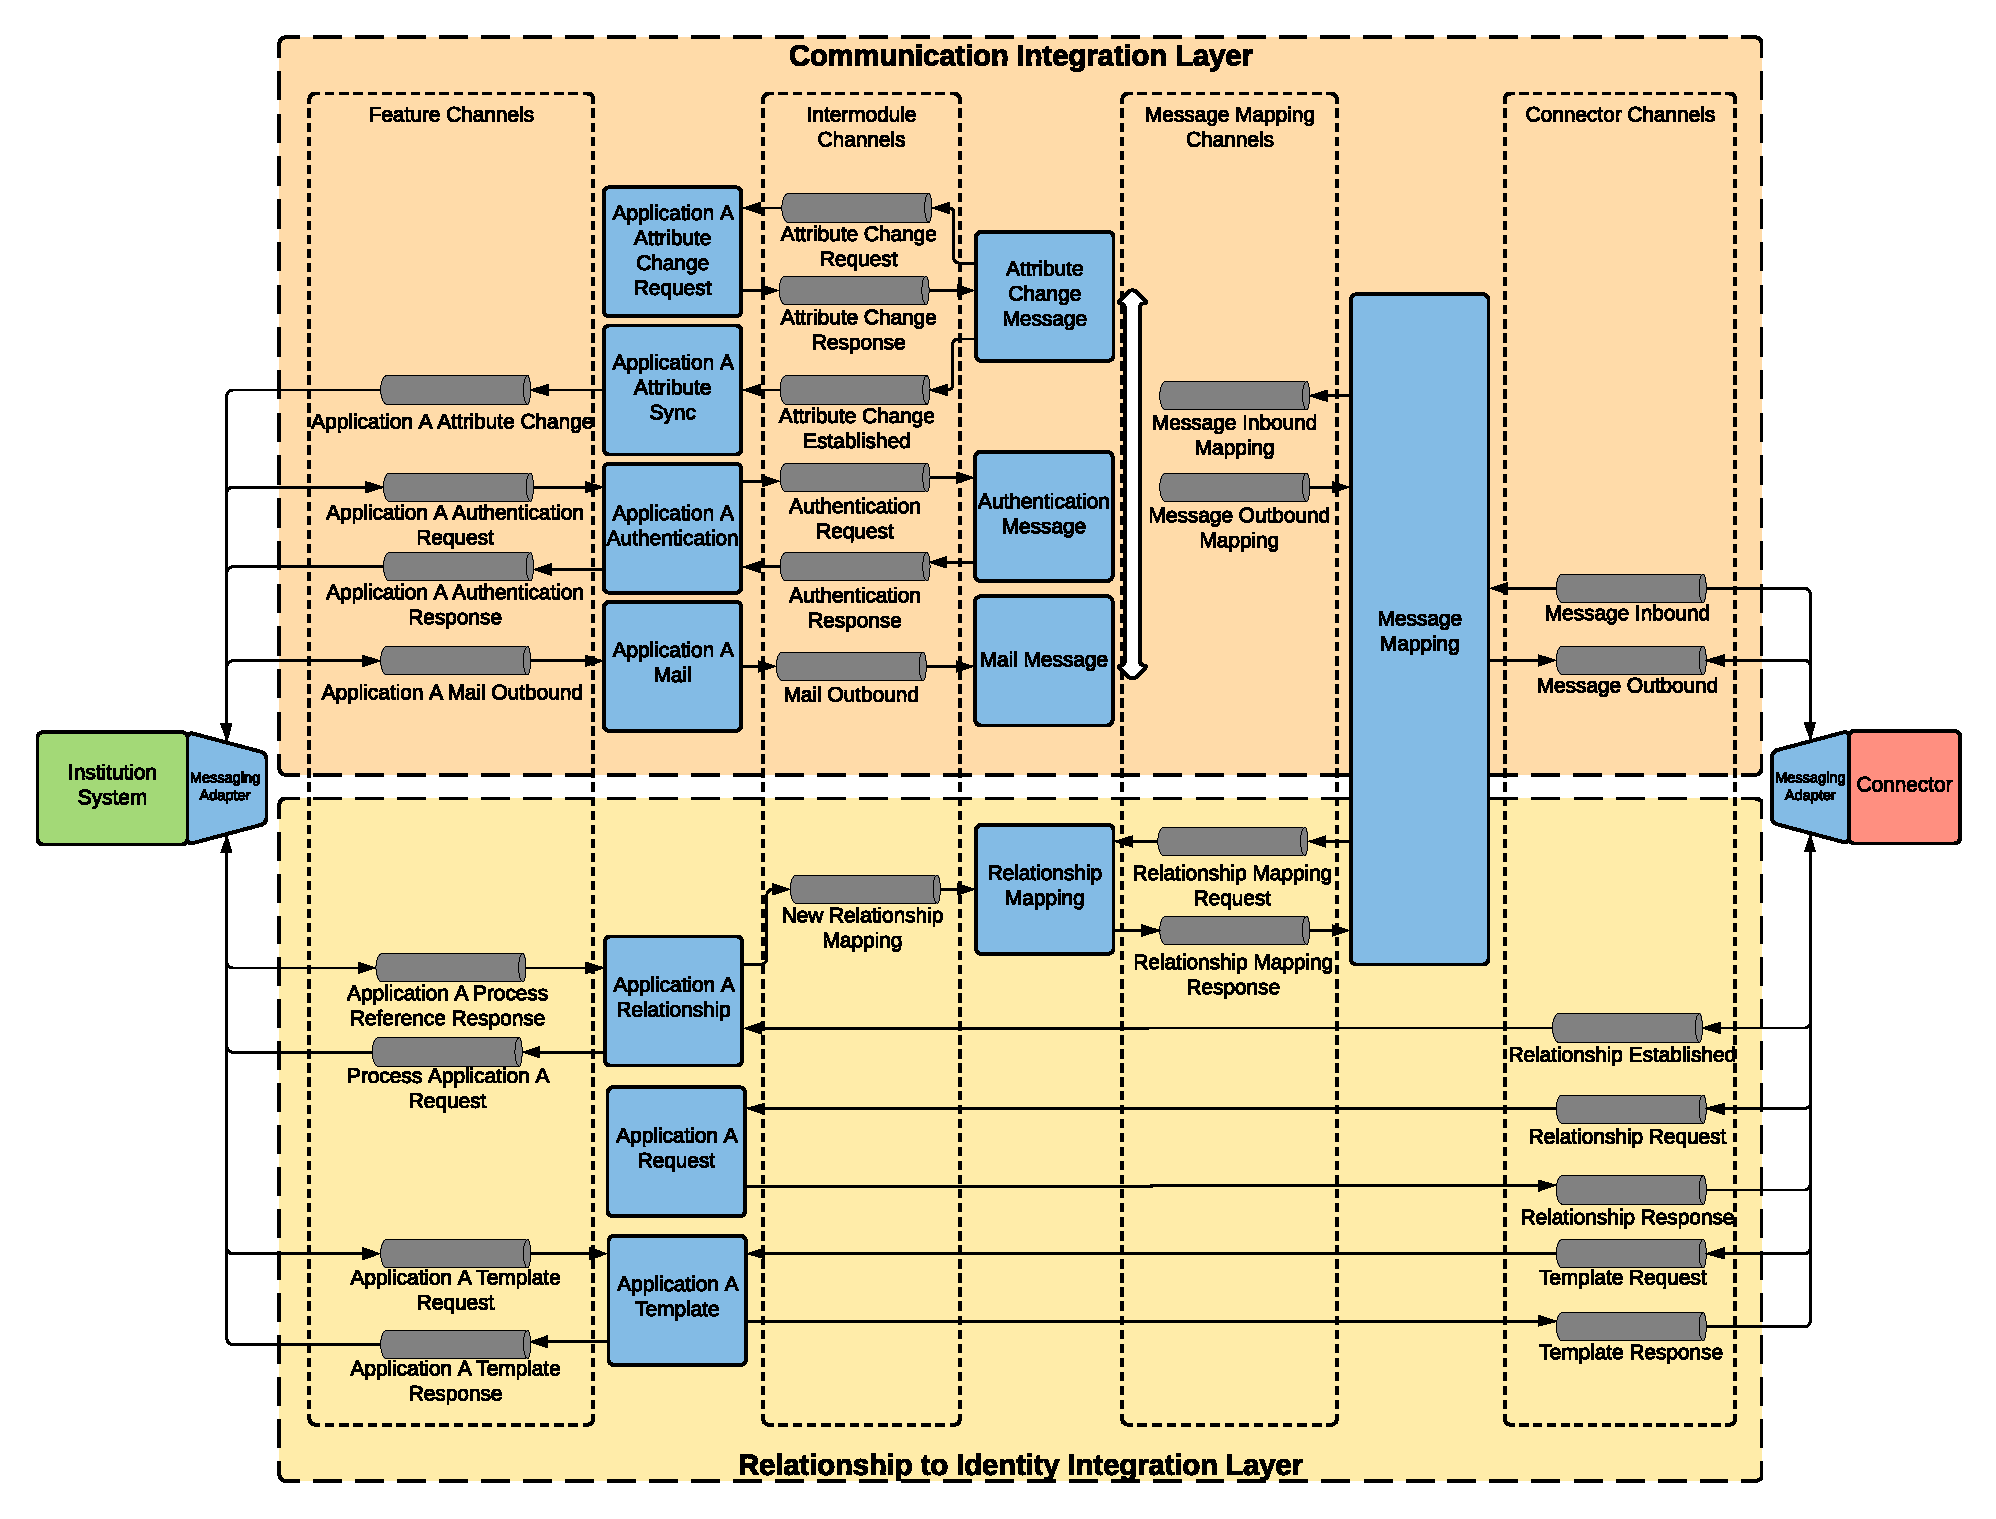
\includegraphics[scale=0.5]{Diagrams/Integration Architecture 2/Technological Integration/2. Messaging Overview.pdf}
\end{center}

The layout of the messaging system is identical to the one presented in section 4.2. Exactly the same type of messages are exchanged with however, a slightly different purpose and content. 

On the "Relationship to Identity Integration Layer", modules exist for establishing the different types of application relationships. For simplification, modules only for an "Application A" are shown. Besides the content and purpose of relationships in this case are different to the relationships of chapter 4, they are processed exactly the same: Each type of relationship request is processed by an individual application request module and each type of established relationship is processed by an individual application relationship module. As the purpose of relationships in this case are applications for administrative services, each module has to be configured appropriately. For an established relationship, instead of issuing the existing system architecture to create a user profile, the application relationship module issues the existing system architecture to process an application based on the attributes shared as part of the relationship. And instead of a user profile ID, the existing system architecture responds with an application process reference ID. This application process reference ID is used in the same way as the user profile ID in section 4.2. Trough the "New Relationship Mapping" channel, it is sent to the relationship mapping module, which maps each relationship to an application process and vice versa.

On the "Communication Integration Layer", the same types of messages are exchanged. However instead of user profile IDs, relationship IDs are mapped to application process reference IDs. In chapter 4, each module connected to the messaging adapter of the institution system was designed to be able to distinguish between different types of user profile IDs in order to for example distinguish a enterprise profile from the profile of a private person. In this case, modules can distinguish between different application types based on the application process reference ID. 



...... Hier muss noch mehr kommen (ausführlicher) .......